\section*{Modeling CRISPR repression using {\tt libSBOLj 2.0}}
We now describe the CRISPR-based repression module and how it can be modeled and encoded using the {\tt libSBOLj 2.0} library. We use bold font in the following text and figure captions to mark available data model in SBOL 2.0. 

\subsection*{CRISPR repression model}
First, consider the CRISPR-based Repression Template \textbf{ModuleDefinition} shown in the center of Figure \ref{SBOL2}. It provides a generic description of CRISPR-based repression behavior. Namely, it includes generic \emph{Cas9}, \emph{guide RNA} (gRNA), and \emph{target} DNA \textbf{FunctionalComponent} instances. It also includes a \emph{genetic production} \textbf{Interaction} that expresses a generic target gene product.  Finally, it includes a \emph{non-covalent binding} \textbf{Interaction} that forms the Cas9/gRNA complex (shown as dashed arrows), which in turn participates in an \emph{inhibition} \textbf{Interaction} to repress the target gene product production (shown with a tee-headed arrow). The CRISPR-based Repression Template is then instantiated to test a particular CRISPR-based repression device, CRPb, by the outer CRPb Characterization Circuit \textbf{ModuleDefinition}.  This outer characterization circuit includes gene \textbf{FunctionalComponents} to produce specific products (i.e., mKate, Gal4VP16, cas9m\_BFP, gRNA\_b, and EYFP), as well as \textbf{FunctionalComponents} for the products themselves.  Next, it includes \emph{genetic production} \textbf{Interactions} connecting the genes to their products, and it has a \emph{stimulation} \textbf{Interaction} that indicates that Gal4VP16 stimulates production of EYFP.  Finally, it uses \textbf{MapsTo} objects (shown as dashed lines) to connect the generic \textbf{FunctionalComponents} in the template to the specific objects in the outer \textbf{ModuleDefinition}.  For example, the outer module indicates that the target protein is EYFP, while the cas9\_gRNA complex is cas9m\_BFP\_gRNA\_b.

\begin{figure}[tbph]
\begin{center}
  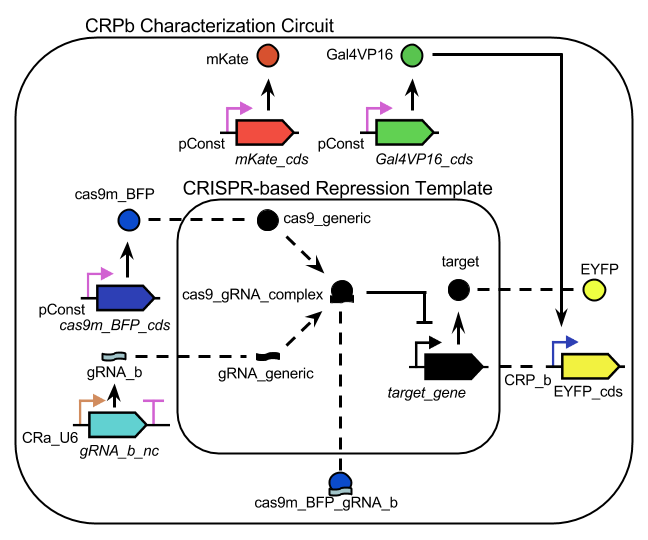
\includegraphics[width=0.95\textwidth]{figures/crispr_repression2} 
\end{center}
\caption{\label{SBOL2} Illustration of a hierarchical CRISPR-based repression module represented in SBOL 2.0 (adapted from Figure 1a in \cite{kiani2014crispr}). The CRISPR-based Repression Template \textbf{ModuleDefinition} describes a generic CRISPR repression circuit that combines a Cas9 protein with a gRNA to form a complex (represented by the dashed arrows) that represses a target gene (represented by the arrow with the tee arrowhead).  These relationships between these \textbf{FunctionalComponents} (instances of \textbf{ComponentDefinitions}) are represented in SBOL 2.0 using \textbf{Interactions}.  This \textbf{Module} is instantiated in the outer CRPb Characterization Circuit \textbf{ModuleDefinition} in order to specify the precise (including \textbf{Sequences} when provided) \textbf{FunctionalComponents}  used for each generic \textbf{FunctionalComponent}. The undirected dashed lines going into the template \textbf{Module} represent \textbf{MapsTo} objects that specify how specific \textbf{FunctionalComponents} replace the generic ones.}
\end{figure}

\subsection*{Encoding using {\tt libSBOLj 2.0}}
Program~\ref{JavaExample} illustrates the use of the {\tt libSBOLj 2.0} library using an excerpt of the Java code to express the CRISPR-based repressor design in SBOL 2.0. First, a new \textbf{SBOLDocument} is created (line 1), and is given a default URI prefix (line 2). At this point, \textbf{ComponentDefinition} and \textbf{Interaction} objects are also created for the CRISPR-based Repression Template \textbf{ModuleDefinition} (not shown).  Then, \textbf{Sequence} objects are created for those sequences provided in \cite{kiani2014crispr}.\footnote{Unfortunately, as usual, not all sequences are provided in the paper.} For example, to create the sequence for the CRP\_b promoter, we call the {\tt createSequence} method with the \emph{displayId} (CRP\_b\_seq), \emph{version} (1.0), the sequence, and the encoding used (line 3).  
Note that this method, as well as other create methods in the library, creates a \emph{compliant URI} that has the following form:
\begin{center}
http://$\langle$prefix$\rangle$/$\langle$displayId$\rangle$/$\langle$version$\rangle$
\end{center}
using the default URI prefix and provided \emph{displayId} and \emph{version}. The \emph{$\langle$prefix$\rangle$} represents a URI for a namespace (for example, {\tt www.sbols.org/CRISPR\_Example}). The author of a \textbf{TopLevel} object, such as the \textbf{Sequence} object we just created, should use a URI prefix that either they own or an organization of which they are a member owns. When using compliant URIs, the owner of a prefix must ensure that the URI of any unique \textbf{TopLevel} object that contains the prefix also contains a unique  \emph{$\langle$displayId$\rangle$} or \emph{$\langle$version$\rangle$} portion. Multiple versions of an SBOL object can exist and would have compliant URIs that contain identical prefixes and displayIds, but each of these URIs would need to end with a unique version. Lastly, the compliant URI of a non-\textbf{TopLevel} object is identical to that of its parent object, except that its displayId is inserted between its parent's displayId and version. This form of compliant URIs is chosen to be easy to read, facilitate debugging, and support a more efficient means of looking up objects and checking URI uniqueness. 

\begin{program*}[ht]
\begin{lstlisting}[language=java,style=highlight]
SBOLDocument doc = new SBOLDocument();
doc.setDefaultURIprefix("http://sbols.org/CRISPR_Example/");
doc.createSequence("CRP_b_seq", "1.0", "GCTCCGAATTTCTCGACAGATCTCATGTGAT...", !!Sequence??.<<>>IUPAC_DNA>><<); 
ComponentDefinition CRP_b = doc.createComponentDefinition("CRP_b", "1.0", !!ComponentDefinition??.<<>>DNA>><<);
CRP_b.addRole(!!SequenceOntology??.<<>>PROMOTER>><<);
CRP_b.addSequence("CRP_b_seq");
doc.createComponentDefinition("EYFP_cds", "1.0", !!ComponentDefinition??.<<>>DNA>><<).addRole(!!SequenceOntology??.<<>>CDS>><<);
ComponentDefinition EYFP_gene = doc.createComponentDefinition("EYFP_gene", "1.0", !!ComponentDefinition??.<<>>DNA>><<);
EYFP_gene.createSequenceConstraint("EYFP_gene_constraint", !!RestrictionType??.<<>>PRECEDES>><<, "CRP_b", "EYFP_cds");
doc.createComponentDefinition("Gal4VP16", "1.0", !!ComponentDefinition??.<<>>PROTEIN>><<);
ModuleDefinition CRPb_circuit = doc.createModuleDefinition("CRPb_characterization_circuit", "1.0");
Interaction EYFP_Activation = CRPb_circuit.createInteraction("EYFP_Activation", 
                                                             !!SystemsBiologyOntology??.<<>>STIMULATION>><<);
EYFP_Activation.createParticipation("GAL4VP16", "Gal4VP16").addRole(!!SystemsBiologyOntology??.<<>>STIMULATOR>><<);
EYFP_Activation.createParticipation("EYFP_gene", "EYFP_gene").addRole(!!SystemsBiologyOntology??.<<>>PROMOTER>><<);
Module Template_Module = CRPb_circuit.createModule("CRISPR_Template", "CRISPR_Template", "1.0");
Template_Module.createMapsTo("EYFP_gene_map", !!RefinementType??.<<>>USELOCAL>><<, "EYFP_gene", "target_gene");
\end{lstlisting}
\caption{\label{JavaExample}Fragments of Java code to produce part of the CRISPR Repression example using {\tt libSBOLj 2.0}.}
\end{program*}

Next, we create \textbf{ComponentDefinition} objects for each element in the module. For example, a \textbf{ComponentDefinition} of DNA type is created for the CRP\_b promoter (lines 4-6).  Note that by using compliant URIs, the sequence can be looked up using its \emph{displayId}, and since no version is provided, it is referenced by its \emph{persistentIdentity} URI (line 6). It is simply its URI without the version when using compliant URIs. The purpose of a persistent identity is to allow an object to refer to the latest version of another object using this URI. The latest version of an object is determined using \emph{semantic versioning} conventions (c.f., {\tt http://semver.org/}).

Next, we create two \textbf{ComponentDefinition} objects, one for the EYFP \emph{coding sequence} (CDS), and one for the EYFP gene (lines 7-8). We use a \textbf{SequenceConstraint} object (line 9) to indicate that the CRP\_b promoter precedes the EYFP CDS, because the sequence for the CDS has not been provided and thus cannot be given an exact \textbf{Range}. Finally, we create a protein type \textbf{ComponentDefinition} for the Gal4VP16 protein (line 10). After all the \textbf{ComponentDefinitions} are created, we create a \textbf{ModuleDefinition} object for the CRPb Characterization Circuit (line 11). 

Next, the \textbf{Interactions} between the components are specified using terms from the \emph{Systems Biology Ontology} (SBO) \cite{Courtot2011}.  One example \textbf{Interaction} is the stimulation of the \texttt{EYFP\_gene} by the Gal4VP16 protein (lines 12-14).  Now, the CRISPR-based Repression Template \textbf{Module} is instantiated and connected to the CRPb Characterization Circuit using \textbf{MapsTo} objects.  
For example, a \textbf{MapsTo} object is used to indicate that the \texttt{target\_gene} in the template should be refined to be the \texttt{EYFP\_gene} specified in the CRPb circuit (line 17).  

As we mentioned previously, the complete repression model is described in the ``RepressionModel.java'' under the libSBOLj examples directory. This example is self-contained in that you can run it to generate the RDF/XML output. Also, SBOL does not provide the specification of a mathematical model directly. It is possible, however, to generate a mathematical model using SBML~\cite{SBML} and the procedure described in~\cite{roehner2015generating}. Then, the SBOL document can reference this generated SBML model.


